\FloatBarrier
\subsection{Presentazione del sistema}
La pagina iniziale è stata studiata per poter esser gestita in maniera semplice ed intuitiva dall'utente.  Tutti i contenuti sono stati suddivisi in aree  per  una  corretta  ed  intuitiva  visualizzazione. 
A  ciascuna sezione   sono   stati associati dei moduli dinamici (figura \ref{Screen:first}):

\begin{itemize}
\item selezione mappa;
\item barra di ricerca persona;
\item visualizzazione mappa o risultati ricerca;
\item visualizzazione/modifica informazioni.
\end{itemize}

\begin{figure}[!htb]
\centering%
\includegraphics[scale=0.5]{FirstScreen.png}%
\caption{Organizzazione pagina iniziale}\label{Screen:first}%
\end{figure}

\FloatBarrier
\subsubsection*{Selezione mappa}
Nell'area "Selezione mappa" è possibile scegliere la mappa da visualizzare(tramite la selezione di un edificio e un suo piano) e la modalità in cui verrà presentata.

\subsubsection*{Barra di ricerca}
Questa barra permette di cercare le persone registrate nel database per ottenere le informazioni sulle stanze da loro occupate. Durante la tipizzazione del nome/cognome all'interno della barra di ricerca, vengono mostrati suggerimenti per velocizzare e rendere più accurato questo servizio (RF07).

\begin{figure}[!htb]
\centering%
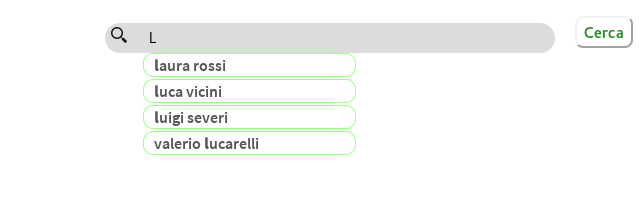
\includegraphics[scale=0.5]{AdvicesScreen.png}%
\caption{Ricerca di persone.}\label{Screen:advices}%
\end{figure}
\FloatBarrier

\subsubsection*{Visualizzazione mappa / risultati ricerca}
In quest'area sono possibili due casi:
\begin{enumerate}
\item viene mostrata la mappa in formao SVG nella modalità selezionata in "Selezione mappa";

\begin{figure}[!htb]
\centering%
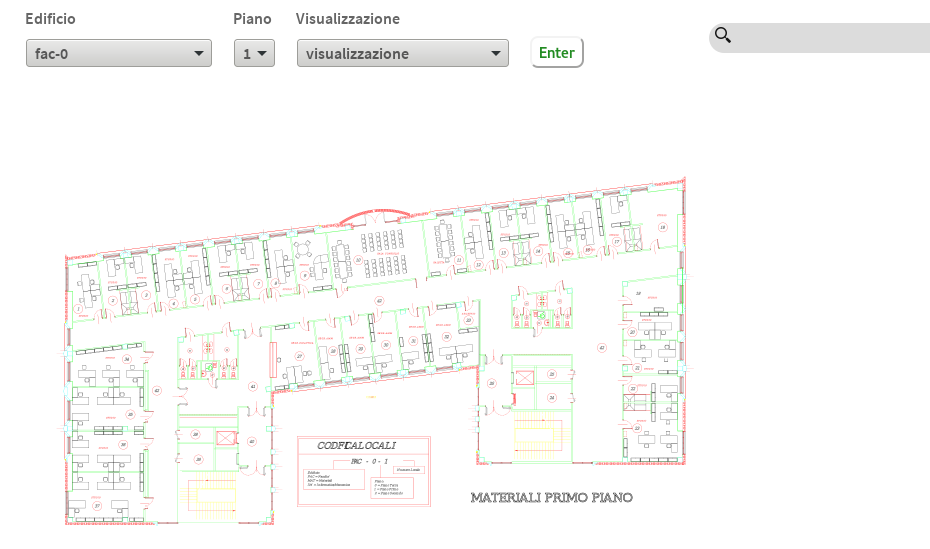
\includegraphics[scale=0.3]{ShowMap.png}
\caption{Esempio di visualizzazione mappa}\label{Screen:showmap}%
\end{figure}
\FloatBarrier

\item viene fatta vedere una lista delle aule occupate dalle persone inserite nella "Barra di ricerca" con le relative informazione.

\begin{figure}[!htb]
\centering%
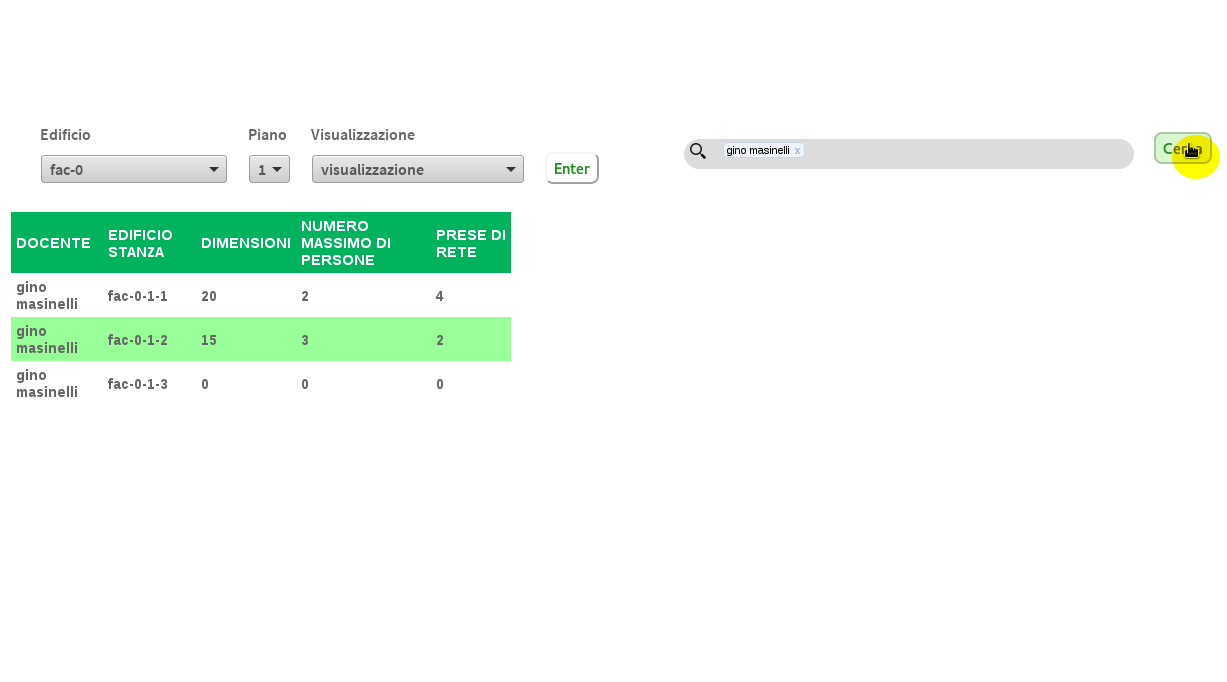
\includegraphics[scale=0.3]{SearchScreen.png}%
\caption{Esempio di risultato della ricerca}\label{Screen:search}%
\end{figure}
\FloatBarrier

\end{enumerate}
\newpage
\subsubsection*{Visualizzazione/modifica informazioni}
La visualizzazione e la modifica delle informazioni relative a stanze o persone selezionate avviene in questa sezione.

\begin{figure}[!htb]
\centering%
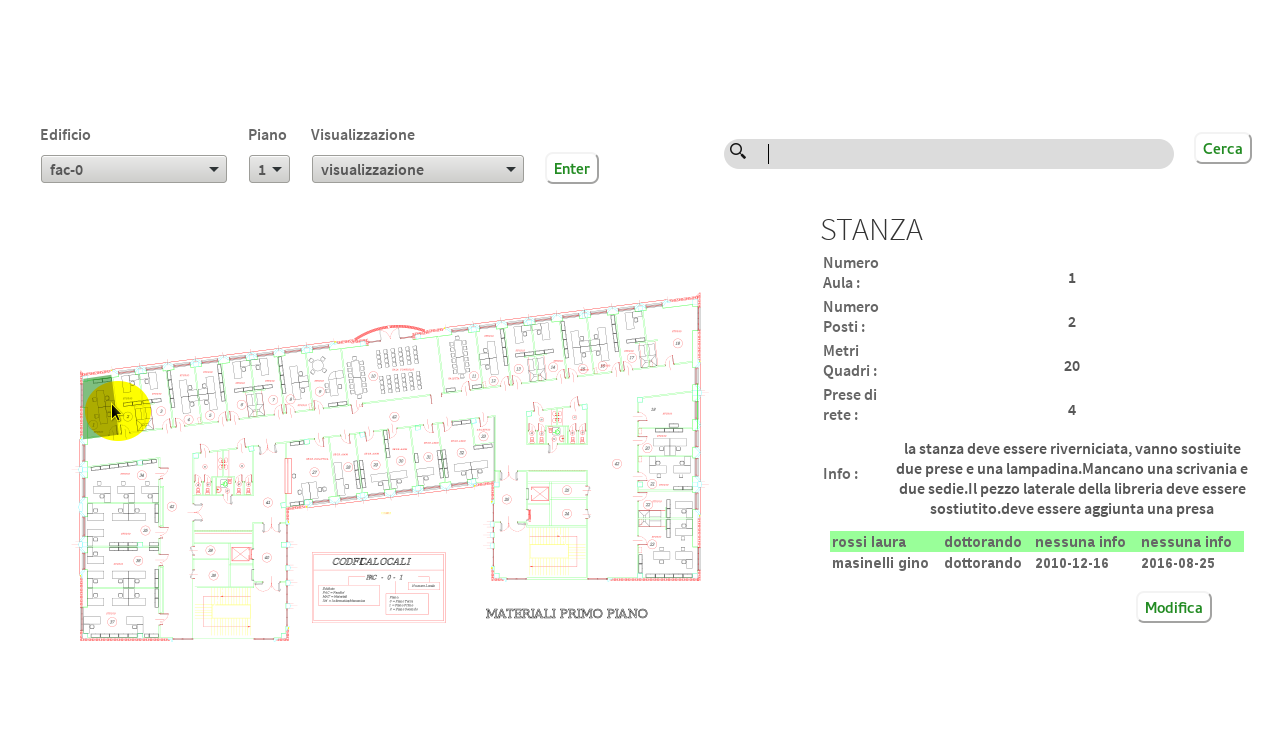
\includegraphics[scale=0.3]{RoomSelScreen.png}
\caption{Esempio di visualizzazione informazioni quando si seleziona una stanza.}\label{Screen:info1}%
\end{figure}

\begin{figure}[!htb]
\centering%
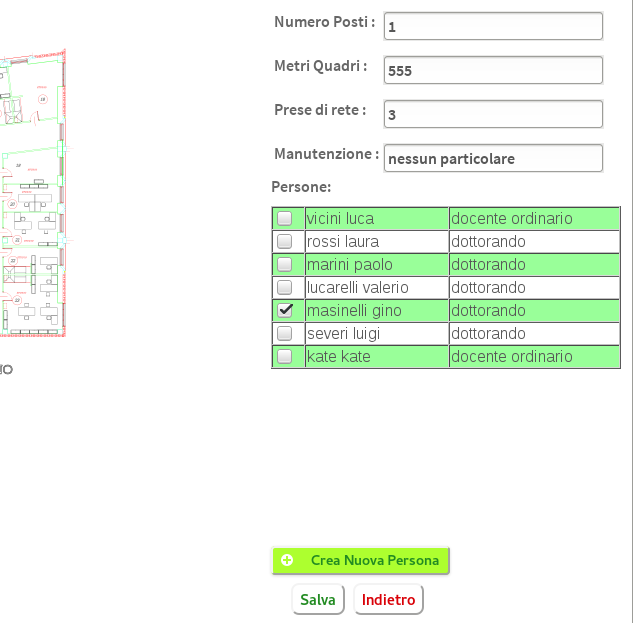
\includegraphics[scale=0.3]{ShowInfo2.png}%
\caption{Esempio di modifica informazioni di una stanza.}\label{Screen:info2}%
\end{figure}
\FloatBarrier

